\chapter{Licht - Materie Wechselwirkung}

\section{lineare und zirkulare Polarisation}

EM-Welle
\begin{equation*}
\Rightarrow \vec{E},\vec{B},\vec{k}
\end{equation*}
\textbf{Definition: } Polarisation $ \widehat{=} $ Richtung von $ \vec{E} $\\
transversale Wellen: $ \ \vec{E} \perp \vec{k} \quad \Leftrightarrow \quad \ \: \vec{E} \cdot \vec{k} = 0 $\\
longitudinale Wellen: $ \vec{E} \parallel \vec{k} \, \quad \Leftrightarrow \quad \vec{E} \times \vec{k} = 0 \quad \Leftrightarrow \quad \left(\vec{E} \cdot \vec{k}\right) \vec{k} = \vec{k}^2 \vec{E} $\\
\lcom{Für die Behauptung, dass EM-Wellen Transversalwellen haben wir die Annahme getroffen, dass wir uns im Vakuum befinden. In Materie ist die Ausbreitungsgeschwindigkeit kleiner als $ c $ und der $ \vec{k} $-Vektor hat eine Komponente parallel zur Ausbreitungsrichtung. $ \Rightarrow $ longitudinale EM-Wellen (eigentlich keine EM-Wellen sondern anderer Name).}\\
zur Vereinfachung nehmen wir an $ \Rightarrow \vec{k} = (0,0,k) $

\subsection{Lineare Polarisation}

\folie{linear polarisierte EM-Welle}
\begin{equation*}
\vec{E} = \ub{E_0 \begin{pmatrix}
\cos \tilde{\varphi} \\ \sin \tilde{\varphi} \\ 0
\end{pmatrix}}_{\vec{E}_0} \cos \left(\omega t - k z + \varphi \right)
\end{equation*}
\emph{Bemerkung:}
\begin{itemize}
	\item Die zwei Polarisationsrichtungen schwingen \textbf{in Phase}.
	\item nur für die linear polarisierte ebene Welle kann der ,,Polarisationsanteil`` $ \vec{E}_0 $ vom ,,Ausbreitungsanteil`` $ \cos (\omega t - \vec{k} \vec{z} + \varphi) $ ab separiert werden
\end{itemize}

\subsection{Zirklulare Polarisation}

\folie{zirkular polarisierte EM-Welle}
\begin{equation*}
\vec{E} = E_0 \begin{pmatrix}
\cos \left(\omega t - kz + \varphi \right) \\ \pm\sin\left(\omega t - k z + \varphi\right) \\ 0
\end{pmatrix}
\end{equation*}
\emph{Bemerkung:}
\begin{itemize}
	\item die zwei Polarisationsrichtungen schwingen um $ \frac{\pi}{2} $ \textbf{Phasen verschoben}, aber haben gleiche Amplitude
\end{itemize}

\subsection{Zusammenhang zwischen linear und zirkular polarisierten Wellen}

\rbox{Jede linear polarisierte Welle kann in zwei entgegengesetzt zirkular polarisierte Wellen halber Amplitude zerlegt werden und umgekehrt.}
\noindent
\emph{Beispiel:} Zerlegung von linearer in zirkulare Polarisation.
$ \cos\left( x + \frac{\pi}{2}\right) + \cos\left( x - \frac{\pi}{2}\right) = 0 $
\begin{align*}
\vec{E}(\vec{x},t) &= A \begin{pmatrix}
\cos\left(\omega t - k z + \varphi\right) \\ 0 \\ 0
\end{pmatrix} \\
&= \frac{A}{2} \begin{pmatrix}
\cos\left(\omega t - k z + \varphi \right) \\ \cos\left(\omega t - k z + \varphi + \frac{\pi}{2}\right) \\ 0
\end{pmatrix} + \frac{A}{2} \begin{pmatrix}
\cos \left(\omega t - k z + \varphi\right) \\ \cos \left(\omega t -  k z + \varphi - \frac{\pi}{2}\right) \\ 0
\end{pmatrix}
\end{align*}

\subsection{Elliptische Polarisation}

Die Spitze des $ \vec{E} $-Feldvektors bewegt sich mit der Frequenz $ \omega $ auf einer Ellipse
\begin{equation*}
\vec{E} = \begin{pmatrix}
E_x \cos(\omega t - k z + \varphi) \\
E_y \cos(\omega t - k z + \varphi \pm \frac{\pi}{2}) \\
0
\end{pmatrix}
\end{equation*}
\emph{Bemerkung:}
\begin{itemize}
	\item die zwei Polarisationsrichtungen schwingen um $ \frac{\pi}{2} $ Phase verschoben UND haben unterschiedliche Amplituden
\end{itemize}

\subsection{Polarisation beim Durchgang durch Materie}

\subsubsection{Doppelbrechung:}

\begin{equation*}
k_x \neq k_y
\end{equation*}
\begin{equation*}
\vec{E}(\vec{x},t) = \begin{pmatrix}
A_x \cos\left(\omega t - \color{black!30!red}k_x\color{black}z + \varphi_x\right) \\ A_y \cos\left(\omega t - \color{black!30!red}k_y\color{black}z + \varphi_y \right) \\ 0
\end{pmatrix}
\end{equation*}

\subsubsection{optische Aktivität}

Die Ausbreitungsgeschwindigkeit bzw. der Wellenvektor für rechts und links zirkulare Polarisation unterschiedlich.

\begin{align*}
\Rightarrow \quad \vec{E}(\vec{x},t) &= \frac{A}{2} \begin{pmatrix}
\cos\left(\omega t - \color{black!30!red}k^+\color{black}z + \varphi\right) \\ \cos\left(\omega t -\color{black!30!red}k^+\color{black}z + \varphi + \frac{\pi}{2}\right) \\ 0
\end{pmatrix} + \frac{A}{2} \begin{pmatrix}
\cos\left(\omega t - \color{black!30!red}k^-\color{black}z + \varphi\right) \\ \cos\left(\omega t - \color{black!30!red}k^-\color{black}z+\varphi-\frac{\pi}{2}\right) \\ 0
\end{pmatrix}\\
&=A \begin{pmatrix}
\cos\left(\delta kz\right) \\ \sin\left(\delta kz\right) \\ 0
\end{pmatrix} \cos\left(\omega t - \overline{k}z + \varphi\right)
\end{align*}
\begin{equation*}
k^+ = \overline{k} + \delta k \qquad k^- = \overline{k} - \delta k
\end{equation*}

\section{Polarisation durch Brechung und Reflexion}

(siehe EX II)

\subsection{Maxwell Gleichungen in Materie}

\begin{equation*}
\tx{div} \vec{D} = \rho_0 \qquad \qquad \tx{div} \vec{B} = 0 \qquad \qquad
\end{equation*}
\begin{equation*}
\tx{rot} \vec{E} = - \prt{}{t} \vec{B} \qquad \tx{rot} \vec{H} = \vec{j}_0 + \prt{}{t} \vec{D}
\end{equation*}
plus:
\begin{align*}
\vec{F} &= q \left(\vec{v} \times \vec{B}\right) \\
\vec{F} &= q \vec{E}
\end{align*}
\begin{equation*}
\rho = \rho_0 + \rho_{\tx{pol}} \equiv \frac{1}{\epsilon} \rho_0 \qquad \vec{j} = \vec{j}_0 + \vec{j}_{\tx{mag}} \equiv \mu \vec{j}_0
\end{equation*}
Es fehlen hier noch einige Zusammenhänge die selbstverständlich immer noch gelten z.B.:
\begin{equation*}
\tx{div} \vec{E} = \frac{1}{\epsilon_0} \rho \qquad \tx{rot} \vec{B} = \mu_0 \vec{j} + \frac{1}{c^2} \prt{}{t} \vec{E} 
\end{equation*}
\begin{equation*}
\vec{D} = \epsilon_0 \vec{E} + \vec{P} \qquad \vec{B} = \mu_0\left(\vec{H} + \vec{M}\right)
\end{equation*}
alle sechs Felder: $\vec D  \vec E \vec P \ \ \vec M \vec H \vec B$ jeweils Maxwell-Gleichungen\\
plus:
\begin{equation*}
\tx{Materialgleichungen z.B.:} \quad \vec{D} (\vec{E}) \ , \ \vec{P}(\vec{E}) \ , \dots
\end{equation*}

\subsection{Erinnerung: Polarisation bei Brechung und Reflexion}

\folie{Brechung und Reflexion bei parallelem und orthogonalem $ \vec{E} $-Feld in der Einfallsebene}\\
\folie{Einfallswinkel und Reflexionswinkel (Brewsterwinkel)}

\subsubsection{Physikalische Ursache: Stetigkeits \& Randbedingungen}

Gewöhnliche partielle Diff-Gleichungen
\begin{enumerate}[$ \Rightarrow $]
	\item viele Lösungen
	\item Anfangsbed, Randbed., Stetigkeitsbed.
\end{enumerate}
\begin{minipage}{.6\linewidth}
	\emph{Beispiele:}
	\begin{itemize}
		\item Metall:
		Randbedingung aus Elektrostatik überlegt 
		\item Ein- und Ausschaltvorgänge bei RLC Gleichungen
		Anfang: Schalter offen, Spule ,,aufgeladen``
		\begin{equation*}
		\Rightarrow I = \frac{U}{(R_i + R)}
		\end{equation*}
		Dann: Schalter schließen $ \Rightarrow U = 0 $
		$ \Rightarrow $ wie verhält sich aber $ I , U_{\tx{Spule}}, \dots $ ?\\
		Energie der Spule ist stetig $ \ \ E_{\tx{Spule}} = \frac{1}{2} L I^2 $
		\begin{equation*}
		\Rightarrow I_{\tx{Spule}} \tx{ stetig}
		\end{equation*}
	\end{itemize}
\end{minipage}%
\begin{minipage}{.4\linewidth}
	\centering
	%t1:
	\begin{tikzpicture}
	\centerarc[pattern = north east lines](0,0)(200:90:2cm);
	\draw[very thick,->] (135:2cm) -- node[anchor=south west] {$ \vec{E} $} ++(135:1.2cm);
	\centerarc[](135:2cm)(135:40:.3cm);
	\node[fill=black,circle,inner sep=.5pt,minimum size=.5pt] at ($ (135:2cm) + (.01,.15) $) {};
	\draw[white] (0,0) -- (0,-1.2);
	\end{tikzpicture}
	%t2:
	%\draw[decoration={aspect=0.3, segment length=3mm, amplitude=3mm,coil},decorate] (-2,0)--(a);
	\begin{tikzpicture}
	\coordinate (u) at (0,0);
	\coordinate (r1) at (1,1.5);
	\coordinate (r2) at (3.5,1.25);
	\coordinate (l) at (3.5,-.25);
	\coordinate (s) at (2.5,.5);
	\draw[thick] ($ (u) + (-.5,.1) $) -- ++(1,0);
	\draw[thick] ($ (u) + (-.4,-.1) $) -- ++(.8,0);
	\draw[thick] ($ (r1) + (0,-.2) $) rectangle node[] {$ R_i $} ($ (r1) + (1,.2) $);
	\draw[thick] ($ (r2) + (-.2,0) $) rectangle node[] {$ R $} ($ (r2) + (.2,-1) $);
	\draw[decoration={aspect=0.5, segment length=2mm, amplitude=2mm,coil},decorate,thick] (l) -- node[right=10pt] {$ L $} ($ (l) + (0,-1) $);
	\node[circle,fill=black,inner sep=1pt,minimum size=1pt] at (s) {};
	\node[circle,fill=black,inner sep=1pt,minimum size=1pt] at ($ (s) + (0,-1) $) {};
	\draw ($ (u) + (0,.11) $) -- (0,1.5) -- (r1);
	\draw ($ (r1) + (1,0) $) -- (3.5,1.5) -- (r2);
	\draw ($ (r2) + (0,-1) $) -- (l);
	\draw ($ (l) + (0,-1) $) -- (3.5,-1.5) -- (0,-1.5) -- ($ (u) + (0,-.1) $);
	\draw ($ (s) + (0,1) $) -- (s);
	\draw ($ (s) + (0,-2) $) -- ($ (s) + (0,-1) $) -- ++(135:1.2cm);
	\node at (-1,0) {$ U $};
	\end{tikzpicture}
\end{minipage}%

% Vorlesung 27.11.18

\subsection{Maxwell-Gleichungen und Stetigkeitsbedingungen}

\lcom{Heute beschäftigen wir uns mit Stetigkeitsbedingungen. Diese sind sehr Wichtig für die Lösung von Differentialgleichungen zur Lösung von Randwertproblemen.}
\begin{comment}% old Version
\begin{align*}
\tx{div} \vec{D} = \rho_0 \quad &\Rightarrow \quad \left(\vec{D}_2 - \vec{D}_1\right) \cdot \vec{n} = \sigma_{\tx{Fläche}}\\[5pt]
\tx{div} \vec{B} = 0 \quad &\Rightarrow \quad \left(\vec{B}_2 - \vec{B}_1\right) \cdot \vec{n} = 0\\
\tx{rot} \vec{E} = - \prt{}{t} \vec{B} \quad &\Rightarrow \quad \left(\vec{E}_2 - \vec{E}_1\right) \times \vec{n} = 0\\
\tx{rot} \vec{H} = \vec{j}_0 + \prt{}{t} \vec{D} \quad &\Rightarrow \quad \left(\vec{H}_2 - \vec{H}_1\right) \times \vec{n} = \vec{j}_{\tx{Fläche}}
\end{align*}
\end{comment}
\begin{equation*}
\begin{split}
&\tx{div} \vec{D} = \rho_0 \\[8pt]
&\tx{div} \vec{B} = 0 \\
&\tx{rot} \vec{E} = - \prt{}{t} \vec{B} \\
&\tx{rot} \vec{H} = \vec{j}_0 + \prt{}{t} \vec{D}
\end{split}
\begin{split}
\quad \Rightarrow \quad \\[8pt]
\quad \Rightarrow \quad \\[8pt]
\quad \Rightarrow \quad \\[8pt]
\quad \Rightarrow \quad 
\end{split}
\begin{split}
\left(\vec{D}_2 - \vec{D}_1\right) \, \cdot \, \vec{n} &= \sigma_{\tx{Fläche}} \\[8pt]
\left(\vec{B}_2 - \vec{B}_1\right) \, \cdot \, \vec{n} &= 0 \\[8pt]
\left(\vec{E}_2 - \vec{E}_1\right) \times \vec{n} &= 0 \\[8pt]
\left(\vec{H}_2 - \vec{H}_1\right) \times \vec{n} &= \vec{j}_{\tx{Fläche}}
\end{split}
\end{equation*}
\begin{enumerate}[$ \Rightarrow $]
	\item Normalkomponenten von $ \vec{B}(\vec{x},t) $ ist stetig
	\item Tangentialkomponente von $ \vec{E}(\vec{x},t) $ ist stetig
\end{enumerate}
\textbf{(nahezu) senkrechten Einfall}\\
$ \alpha,\beta \approx 0 $\\

\begin{minipage}{.05\linewidth}
	$ \perp : $ \\\\[5pt] $ \parallel : $
\end{minipage}%
\begin{minipage}{.45\linewidth}
	\centering
	Reflexion
	\begin{equation*}
	E_{\tx{ref} \perp} = - E_{\tx{ein} \perp} \frac{n_2 - n_1}{n_2 + n_1}
	\end{equation*}
	\begin{equation*}
	\phantom{-} \, E_{\tx{ref} \parallel} = \phantom{-} E_{\tx{ein} \parallel} \, \frac{n_2 - n_1}{n_2 + n_1} \ \ \,
	\end{equation*}
	\vspace{10pt}
\end{minipage}\nolinebreak%
\begin{minipage}{.45\linewidth}
	\centering
	Transmission
	\begin{equation*}
	E_{\tx{trans} \perp} = E_{\tx{ein} \perp} \frac{2 n_1}{n_2 + n_1}
	\end{equation*}
	\begin{equation*}
	E_{\tx{trans} \parallel} = E_{\tx{ein} \parallel} \frac{2 n_1}{n_2 + n_1}
	\end{equation*}
	\vspace{10pt}
\end{minipage}%
\\
Betrachtung für senkrechten Einfall\\
\folie{Stetigkeitsbed. bei senkrechtem Einfall}
\begin{enumerate}[(1)]
	\item $ \perp $ und $ \parallel $ sind identisch $ \Rightarrow $ wähle $ \perp $
	\item Aus Stetigkeit der Tangentialkomponenten von $ E $
	\begin{equation*}
	E_{I} = E_{II}
	\end{equation*}
	\begin{equation*}
	\Rightarrow \qquad E_{\tx{ein} \perp} + E_{\tx{ref} \perp} = E_{\tx{trans} \perp}
	\end{equation*}
	(aus Gauß Zylinder folgt die Gleichheit der E Felder auf einer Seite mit dem E Feld auf der anderen Seite)
	\item Stetigkeit des Energieflusses\\
	\folie{Stetigkeits an Randflächen}
	\begin{equation*}
	\Rightarrow \qquad I_{\tx{ein}} = I_{\tx{ref}} + I_{\tx{trans}}
	\end{equation*}
	\item $ I = n c_0 \epsilon_0 E^2 $
	\begin{equation*}
	\Rightarrow \qquad n_1 (E_{\tx{ein} \perp})^2 = n_1 (E_{\tx{ref} \perp})^2 + n_2 (E_{\tx{trans} \perp})^2
	\end{equation*}
\end{enumerate}
$ \Rightarrow $ Lösungen wie oben

\subsection{Warum war es ,,erlaubt`` mit ebenen Wellen zu rechnen ?}

\begin{enumerate}[(1)]
	\item Lösungen im homogenen Raum, Raum kann begrenzt sein
	\item Grenzfälle $ \rightarrow $ Lösungen in den jeweiligen Teilräumen, wurden durch Stetigkeitsbed. angeschlossen.
	\item Maxwell-Gleichungen sind linear $ \leftrightarrow $ Superpositionsprinzip.\\[5pt]
	spezielle Lösung:
	\begin{equation*}
	\vec{E}(\vec{x},t) = \vec{E}_0 e^{i(\vec{k} \vec{x} - \omega t)} \qquad \tx{ mit } \omega(\vec{k})
	\end{equation*}
	$ \vec{k} $ als Parameter zum ,,numerieren`` der Lösungen\\[5pt]
	allgemeine Lösung:
	\begin{eqnarray}
	\vec{E}(\vec{x},t) = \int \vec{E}_0(\vec{k}) e^{i(\vec{k} \vec{x} - \omega(\vec{k}) t)} \dd \vec{k}
	\end{eqnarray}
\end{enumerate}
$ \Rightarrow $ Allgemein:
\begin{equation*}
\vec{E}_I(\vec{x}_{\tx{Grenzfläche}},t) = \vec{E}_{II} (\vec{x}_{\tx{Grenzfläche}},t)
\end{equation*}
speziell:
\begin{equation*}
\vec{E}(\vec{x},t,p)
\end{equation*}
allgemein:
\begin{equation*}
\vec{E}(\vec{x},t) = \int \vec{f}(p) \vec{E}(\vec{x},t,p) \dd p
\end{equation*}

\section{Maxwell-Gl. in Materie, komplexer Brechungsindex}

\begin{equation*}
\tx{\lcom{\mau \ Im folgenden Kapitel tauchen oft $ \mu $ und $ \epsilon $ auf. Gemeint sind hier aber oft $ \mu_r $ und $ \epsilon_r $ \mau}}
\end{equation*}
Vereinfachung: $ \mu = 1 \ \tx{ eigentlich } \ \mu_r \qquad \vec{B} = \mu_o \vec{H} $

\subsection{Polarisation eines Dielektrikums}

\textbf{phänomenologisch/makroskopisch:}
\begin{equation*}
\vec{D} = \epsilon_0 \vec{E} + \vec{P}
\end{equation*}
allgemein gültig, bis auf:
\lcom{Die Einschränkung der Maxwellgleichungen in Materie sind nur Mittlungen des Mikroskopische Bildes in eine fast Makroskopischen Bereich. Daraus ergibt sich die Einschränkung: Wenn unser Beobachtungsbereich zu klein wird, sind diese Mittlungen nicht mehr gültig.}
\begin{equation*}
\vec{P} = \epsilon_0 \overset{\circ}{\chi} \vec{E} + \dots
\end{equation*}
häufig gültig\\[5pt]
lineare, isotrope Medien
\begin{equation*}
\vec{D} = \epsilon_0 \vec{E} + \vec{P} = \epsilon_0 \epsilon \vec{E} \qquad \vec{P} = \epsilon_0 \chi \vec{E} = \epsilon_0 (\epsilon - 1) \vec{E}
\end{equation*}
$ \chi : $ dielektrische Suszeptibilität $ \chi_e = (\epsilon - 1) \ \tx{ eigentlich } \ = (\epsilon_r - 1) $\\[5pt]
mikroskopisch:
\begin{equation*}
\vec{d} = \alpha \vec{E}
\end{equation*}
$ \vec{d} : $ induziertes Dipolmoment\\
$ \alpha : $ Polarisierbarkeit

\subsection{Ensemble unabhängiger induzierter Dipolmomente}

\begin{equation*}
\vec{P} = \frac{1}{V} \sum_i \vec{d}_i \quad \rightarrow \quad \frac{N}{V} \vec{d} \quad \tx{da sich alle Objekte gleich verhalten}
\end{equation*}
\begin{equation*}
\rightarrow \qquad \chi = \frac{1}{\epsilon_0} \frac{N}{V} \alpha \quad \equiv \epsilon - 1 \ (\epsilon_r - 1)
\end{equation*}
\lcom{Gilt bei Gasen gut, bei Festkörpern aufgrund von Dipol-Dipol-Wechselwirkungen nicht mehr gut.}

\subsection{Lorenz-Lorentz-Oszillatormodell}

\folie{Lorenz-Lorentz-Oszillatormodell für die Polarisation}
\begin{equation*}
\Rightarrow \quad \hat{\epsilon} = \epsilon' + i \epsilon''
\end{equation*}
\lcom{Im Mitschrieb steht hier mehr zum Thema}

\subsection{Wellengleichung in Materie}

Materie $ \Rightarrow \rho \neq 0 $
\begin{equation*}
\Rightarrow \quad \tx{div} \vec{E} \neq 0
\end{equation*}
$ \Rightarrow $ Aus $ \tx{div} \vec{E} = 0 $ folgte das eine EM-Welle im Vakuum transversal sind. Dies muss  also nicht mehr so sein.\\[5pt]
Unter Verwendung von
\begin{enumerate}[(1)]
	\item \begin{equation*}
	\tx{rot rot} \vec{E} \custoup{\rightarrow}{=}{\mathclap{\tx{MW}}} - \prt{}{t} \tx{rot} \vec{B} \custoup{\rightarrow}{=}{\mathclap{\mu = 1}} - \mu_0 \prt{}{t} \tx{rot} \vec{H} \custoup{\rightarrow}{=}{\mathclap{\tx{MW}}} - \mu_0 \prt{^2}{t^2} \vec{D}
	\end{equation*}
	\item \begin{equation*}
	\tx{rot rot} \vec{E} = - \vabla^2 \vec{E} + \tx{grad div} \vec{E}
	\end{equation*}
\end{enumerate}
\begin{equation*}
\Rightarrow \qquad \rmbox{\vabla^2 \vec{E} - \frac{1}{c_0^2} \prt{^2}{t^2} \frac{\vec{D}}{\epsilon_0} - \tx{grad div} \vec{E} = 0}
\end{equation*}
\color{black!20!red} $ \tx{grad div} \vec{E} $ ist wegen $ \tx{div} \vec{E} \neq 0 $ \color{black}

\subsection{Wellengleichung in Materie in komplexer Schreibweise}
\begin{equation*}
\hat{\vec{D}} = \epsilon_0 \hat{\epsilon} \hat{\vec{E}} \qquad \hat{\epsilon} = \epsilon' + i \epsilon''
\end{equation*}
\begin{equation*}
\Rightarrow \qquad \vabla^2 \vec{E} - \frac{1}{c_0} \hat{\epsilon} \prt{^2}{t^2} \vec{E} - \tx{grad div} \vec{E} = 0
\end{equation*}
\begin{enumerate}[(1)]
	\item Einsetzen:
	\begin{equation*}
	\vec{E} = \hat{\vec{E}}_0 \tx{exp} \left[i (\hat{\vec{k}} \vec{x} - \omega t)\right] \qquad \hat{\vec{k}} = \vec{k}' + i \vec{k}''
	\end{equation*}
	\item Ausführen der Differentiale
	\begin{equation*}
	\tx{div} \vec{E} = \begin{pmatrix}
	\prt{}{x} \\ \prt{}{y} \\ \prt{}{z}
	\end{pmatrix} \cdot \hat{\vec{E}}_0 e^{i(\hat{\vec{k}} \vec{x} - \omega t)} = \begin{pmatrix}
	i \hat{k}_x \\ i \hat{k}_y \\ i \hat{k}_z
	\end{pmatrix} \cdot \hat{\vec{E}}_0 e^{i(\hat{\vec{k}} \vec{x - \omega t})} 
	\end{equation*}
	und kürzen des Phasenfaktors
	\begin{align*}
	\tx{div} \vec{E} \quad &\rightarrow \quad i \hat{\vec{k}} \cdot \hat{\vec{E}}_0 \\
	\tx{rot} \vec{E} \quad &\rightarrow \quad i \hat{\vec{k}} \times \hat{\vec{E}}_0 \\
	\vabla^2 \vec{E} \quad &\rightarrow \quad - \left(\hat{\vec{k}} \cdot \hat{\vec{k}}\right) \hat{\vec{E}}_0 \\
	\tx{grad} (\tx{div} \vec{E}) \quad &\rightarrow \quad - \left(\hat{\vec{k}} \cdot \hat{\vec{E}}_0\right) \hat{\vec{k}}\\
	\prt{^2}{t^2} \vec{E} \quad &\rightarrow \quad - \omega^2 \hat{\vec{E}}_0
	\end{align*}
	\item Lösung
	\begin{equation*}
	\Rightarrow \qquad \rmbox{- \left(\hat{\vec{k}}^2\right) \hat{\vec{E}}_0 + \frac{\omega^2}{c_0^2} \hat{\epsilon} \hat{\vec{E}}_0 + \left(\hat{\vec{k}} \cdot \hat{\vec{E}}_0\right) \hat{\vec{k}} = 0 }
	\end{equation*}
\end{enumerate}
Beachte:\\
$ \hat{\vec{k}}^2 $ ist \textbf{nicht} das Betragsquadrat
\begin{equation*}
\hat{\vec{k}}^2 = \vec{k}'^2 - \vec{k}''^2 + 2 i \vec{k}' \cdot \vec{k}''
\end{equation*}

\subsubsection{Was bedeutet $ \hat{\vec{k}} = \vec{k}' + i \vec{k}'' $ ?}

\begin{equation*}
e^{i(\hat{\vec{k}} \vec{x} - \omega t)} = e^{i \vec{k}'' \vec{x}} e^{i(\vec{k}' \vec{x} - \omega t)}
\end{equation*}
Teil mit $ \vec{k}'' : $ Dämpfung, Absorption der Welle beim Durchgang durch Materie $ I(x) = I_0 e^{-2 |k''| x} $\\
Teil mit $ \vec{k}' : $ Ausbreitung der Welle mit $ \lambda = \frac{2 \pi}{k'} $
\emph{Bemerkung:}\\
harmonischer Oszillator: $ \hat{\omega} = \omega - i \delta $\\
$ e^{i\hat{\omega t}} = e^{-\delta t} e^{-i \omega t} $\\
$ \delta $ ist die Dämpfung

\subsection{Transversale Lösungen}

transversal $ \Leftrightarrow \quad \hat{\vec{k}} \perp \hat{\vec{E}}_0 $ 
\begin{equation*}
\Rightarrow \quad \rmbox{\hat{\vec{k}} \cdot \hat{\vec{E}}_0 = 0}
\end{equation*}
\begin{equation*}
\Rightarrow \quad \hat{\vec{k}}^2 \hat{\vec{E}}_0 + \frac{\omega^2}{c_0^2} \hat{\epsilon} \hat{\vec{E}}_0 = 0
\end{equation*}
\begin{equation*}
\Rightarrow \quad \rmbox{\hat{\vec{k}}^2 = \frac{\omega^2}{c_0^2} \hat{\epsilon}}
\end{equation*}
\begin{equation*}
\Rightarrow \quad \rmbox{\omega(\hat{\vec{k}}) = c_0 \sqrt{\frac{\hat{\vec{k}}^2}{\hat{\epsilon}}}}
\end{equation*}
Real- und Imaginärteil von $ \hat{\vec{k}} $ sind verknüpft mit Real- und Imaginärteil von $ \hat{\epsilon} $

\subsection{Komplexwertiger Brechungsindex}

\begin{equation*}
\hat{n} = n + i K = \sqrt{\hat{\epsilon}}
\end{equation*}
$ n : $ Brechungsindex\\
$ K : $ Extinktionskoeffizient
\begin{align*}
\Rightarrow \quad 2 n^2 &= \sqrt{\epsilon'^2 + \epsilon''^2} + \epsilon'\\
2 K^2 &= \sqrt{\epsilon'^2 + \epsilon''^2} - \epsilon'
\end{align*}
\begin{equation*}
\Rightarrow \quad \rmbox{\sqrt{\hat{\vec{k}}^2 } = \frac{\omega}{c_0} \hat{n}}
\end{equation*}

\subsection{Lösung für kleine imaginäre Anteile. (schwache Dämpfung bzw Absorbtion)}

Im allgemeinen ist die Lösung nicht einfach, da hier die Wurzeln aus komplexen Zahlen gezogen werden. Deshalb betrachten wir hier die Lösung für kleine imaginäre Anteile.\\
$ k'' \ll k' \quad K \ll n \quad \epsilon'' \ll \epsilon' $
\begin{align*}
2n^2 &= \sqrt{\epsilon'^2 + \epsilon''^2} + \epsilon' \cong \epsilon' \left(1 + \frac{1}{2} \frac{\epsilon''^2}{\epsilon'^2}\right) + \epsilon' \approx 2 \epsilon' \\
2K^2 &= \sqrt{\epsilon'^2 + \epsilon''^2} - \epsilon' \cong \epsilon' \left(1 + \frac{1}{2} \frac{\epsilon''^2}{\epsilon'^2}\right) - \epsilon' \approx \frac{1}{2} \frac{\epsilon''^2}{\epsilon'} = \frac{1}{2} \frac{\epsilon''^2}{n^2}
\end{align*}
\begin{equation*}
\Rightarrow \quad \rmbox{n = \sqrt{\epsilon'} \qquad K = \frac{\epsilon''}{2n}}
\end{equation*}
Was den Wellenvektor angeht erhalten wir:
\begin{equation*}
\sqrt{\hat{\vec{k}}^2} = \sqrt{\vec{k}'^2 - \vec{k}''^2 + 2 i \vec{k}' \cdot \vec{k}''} \approx | \vec{k}' | + i \frac{\vec{k}' \cdot \vec{k}''}{|\vec{k}'|}
\end{equation*}
\begin{equation*}
\Rightarrow \quad |\vec{k}'|  + i \frac{\vec{k}' \cdot \vec{k}''}{|\vec{k}'|} = \frac{\omega}{c_0} (n + i K)
\end{equation*}
\textbf{Physikalische Interpretation}\\[5pt]
Der Realteil von $\epsilon'$ führt zu einer Ausbreitungsgeschwindigkeit $ c = \frac{c_0}{\sqrt{\epsilon'}} $\\
Der Imaginärteil von $\epsilon'$ führt zu einer Dämpfung/Absorption der Welle.\\
$\rightarrow$ In Materie gibt es transversale EM-Wellen mit $ c = \frac{c_0}{\sqrt{\epsilon'}}$ (falls $c\leq c_0$)

% Vorlesung 28.11.18

\subsection{Evaneszente Welle}

\subsubsection{Totalreflektion}

\folie{Evaneszente Welle}\\
$ \alpha \ge \alpha_T \Rightarrow $ keine Wellenausbreitung im optisch dünneren Medium\\[5pt]
Das bedeutet nicht, dass keine el.-mag.-Felder in diesen Bereich eindringen.\\
\folie{Felder treten in Medium ein.}\\
\lcom{Die Felder sind jedoch so schwach, dass sie nach großem Abstand nicht mehr Messbar sind. Sie klingen mit der Einhüllenden $ e^{i k''} $ ab. $ k' $ ist null, da es sich nur um EM-Felder handelt und nicht um eine sich ausbreitende Welle.}\\
\versuch{Übertragung von Evaneszenten Wellen durch zwei Prismen mit geringem Abstand.}
\textbf{Beobachtung:}\\
Die Evaneszente Welle kann ins zweite Prisma eindringen und sich dort ausbreiten.\\
\textbf{Theorie:}\\
Prisma: $ \hat{\epsilon} = \epsilon' + i \epsilon''  \qquad \epsilon' \gg \epsilon''$\\
Das Licht im Prisma wird nur schwach gedämpft. Es ist für Mikrowellen transparent so wie Glas für sichtbares Licht.\\
Vereinfachung:
\begin{equation*}
\epsilon'' = 0
\end{equation*}
Beachte: I.A. nicht $ k'' = 0 $\\[5pt]
Frage: Kann es ein $ \hat{\vec{k}} $ geben, der komplex bzw. imaginär ist?
\begin{equation*}
\hat{\vec{k}}^2 = \frac{\omega^2}{c_0^2} \epsilon' = \vec{k}'^2 - \vec{k}''^2 + 2 i \vec{k}' \cdot \vec{k}''
\end{equation*}
Für sichtbares Licht im Vakuum gilt:
\begin{equation*}
\epsilon' > 0
\end{equation*}
\begin{equation*}
\Rightarrow \quad \vec{k}'^2 - \vec{k}''^2 + 2 i \vec{k}' \cdot \vec{k}'' > 0
\end{equation*}
Lösung 1: Der Normalfall der Wellenausbreitung
\begin{equation*}
\vec{k}'' = 0
\end{equation*}
Lösung 2: Evaneszente Welle
\begin{equation*}
\vec{k}'' > 0 \ \tx{aber} \ \vec{k}' \perp \vec{k}''
\end{equation*}
\begin{equation*}
\Rightarrow \quad \vec{k}'^2 - \vec{k}''^2 > 0
\end{equation*}
\emph{Beispiel:} \textbf{Totalreflexion mit $ \beta = 90 ^\circ $}\\
$ x $-Achse in Richtung der Ausbreitung der Totalreflektierten, $ z $-Achse orthogonal dazu in Richtung des dünneren Mediums $ n_2 $,\\
\lcom{Die $ \vec{k}' $ Komponente ist bei der Totalreflexion parallel zur Oberfläche des Mediums.}\\[5pt]
\textbf{einfallende Welle:}\\
normale Ausbreitung
\begin{equation*}
\hat{\vec{k}}_1 = \vec{k}_1 + i 0
\end{equation*}
\begin{equation*}
\Rightarrow \quad k_1^2 = \frac{\omega^2}{c_0^2} n_1^2 \qquad (k_1: \tx{ Betrag von } \hat{\vec{k}}_1)
\end{equation*}
aus der Geometrie folgt:
\begin{equation*}
k_{1,x} = k_1 \sin\alpha
\end{equation*}
\begin{equation*}
\Rightarrow \quad k_{1,x}^2 = \frac{\omega^2}{c_0^2} n_1^2 \sin^2 \alpha
\end{equation*}
\textbf{ausfallende Welle:}
\begin{equation*}
\hat{\vec{k}}_2 = \begin{pmatrix}
k_{2,x} \\ 0 \\ i k_{2,z}
\end{pmatrix} \quad \Rightarrow \quad \begin{array}{c}
\vec{k}' = (k_{2,x} , 0 , 0) \\ \vec{k}'' = (0 , 0 , k_{2,z})
\end{array}
\end{equation*}
\begin{equation*}
\Rightarrow \quad \hat{\vec{k}}_2^2 = \frac{\omega^2}{c_0^2} n_2^2 = \vec{k}_2'^2 - \vec{k}_2''^2 = k_{2,x}^2 - k_{2,z}^2 > 0
\end{equation*}
\begin{equation*}
\frac{\omega^2}{c_0^2} n_2^2 = k_{2,x}^2 - k_{2,z}^2 > 0
\end{equation*}
Brechungsgesetz: $ n_1 \sin\alpha = n_2 $
\begin{equation*}
\Rightarrow \quad \custo{\leftarrow}{k_{1,x}^2}{\tx{\color{red} > 0 \color{black}}} = k_{2,x}^2 - k_{2,z}^2 \color{red} >0 \color{black}
\end{equation*}
\begin{flushright}
	\vspace{-20pt}
	\color{red} Q.E.D. \color{black}
\end{flushright}
$ \Rightarrow $ Im Falle der Totalreflexion existiert eine evaneszente Welle \mau

\section{Streuung, Spektren und Verwandtes}

\subsection{Grobe Einteilung}

Materiewelle
\begin{itemize}
	\item \textbf{reflektierend} = Licht wird \textbf{gerichtet} zurückgestrahlt
	\item \textbf{streuend} = Licht wird \textbf{ungerichtet} zurückgestrahlt
\end{itemize}
Materie ist
\begin{itemize}
	\item \textbf{absorbierend} = Licht wird \textbf{verschluckt}
	\item \textbf{durchsichtig} = Licht wird \textbf{durchgelassen}
	\item \textbf{transparent} = Licht wird \textbf{teilweise durchgelassen}, \textbf{teils absorbiert} und/oder \textbf{teil gestreut}
\end{itemize}

\subsection{Physikalische Prozesse: Grundgedanken}

\begin{enumerate}[A)]
	\item \textbf{ elastischer/inelastischer Stoß $ \rightarrow $ Streuung}\\
	\folie{zur Streuung an Teilchen}\\
	wie beim Billard\\[5pt]
	\emph{Beispiel:} Lichtstreuung, Streuung am Photon
	\begin{itemize}
		\item Rayleigh-Streuung: elastische Streuung von Photonen an gebundenen Elektronen
		\item Thomson-Streuung: elastische Streuung an ,,quasi freien`` Elektronen
		\lcom{,,quasi frei``: eventuell gebunden aber winzige Bindungsenergie im Vergleich zur Energie der einfallenden Strahlung.}
		\item Compton-Streuung: inelastische Streuung an ,,quasi freien`` Elektronen\\
		relativistisches Billard
		\item Raman-Streuung: inelastische Streuung aufgrund eines inelastischen Stoßes
		\item Mie-Streuung, Brillouin-Streuung, $ \dots $
	\end{itemize}
	\emph{Beispiel:} andere Teilchen
	\begin{itemize}
		\item Elektronenstreuung
		\item Neutronenstreuung
		\item geladene Teilchen: Rutherford-Streuung, Mott-Streuung
	\end{itemize}
	\item \textbf{Anregung/Abregung}\\
	Genereller Ablauf:\\
	\textbf{Anregung} des Systems durch Licht, Stöße oder Wärme $ \rightarrow $ \textbf{Lebensdauer der Anregung} $ \rightarrow $ \textbf{Abregung} des Systems als Licht, aussenden eines Teilchens, Wärme $ \dots $\\[5pt]
	\emph{Beispiel:}
	\begin{itemize}
		\item Absorption: ein Photon wird absorbiert
		\begin{equation*}
		\hbar \omega \rightarrow \Delta E_{\tx{System}}
		\end{equation*}
		\item spontane Emission, Luminanz
		\begin{equation*}
		\Delta E_{\tx{System}} \rightarrow \hbar \omega
		\end{equation*}
		Fluoreszenz: Lebensdauer Kurz ps bis ns \\
		Phosphoreszenz: Lebensdauer deutlich länger als ns \\
		\item Stimulierte Emission:
		\begin{equation*}
		\hbar \omega + \Delta E_{\tx{System}} \rightarrow 2 \hbar \omega
		\end{equation*}
		\lcom{Aus einem Angeregten System und einem einfallenden Photon entstehen zwei kohärente Photonen.}
		\item Photoeffekt:
		\begin{equation*}
		\hbar \omega \rightarrow E_{e^-}
		\end{equation*}
	\end{itemize}
\end{enumerate}

\subsection{Wirkungsquerschnitt (W.Q.S.)}

Üblicherweise als differentieller W.Q.S. (entspricht geometrisch einer Streuung)
\begin{equation*}
\frac{\dd^2 \sigma}{\dd \Omega \dd E}
\end{equation*}
\lcom{Der W.Q.S. ist ein maß dafür wie sehr ein System Streut.}\\
\folie{Streuung und Wirkungsquerschnitt}\\
\lcom{Hierbei wird die Kugel an der Gestreut wird in kleine Flächenelemente geteilt: Raumwinkel-Einheiten.}\\
\folie{Streuung von Teilchen an Materie (Atomen)}

\subsection{Energie und Impulserhaltung}
$ \Rightarrow $ Betrachtung im Energiediagramm\\[5pt]
häufig: System durch diskrete Energieniveaus Beschrieben.\\[5pt]
\folie{Energiediagramme Absorption und ,,dips`` im Frequenz-Intensität Diagramm}\\
\folie{Energiediagramme bei elastischer Streuung}\\
\folie{Energiediagramme bei inelastischen Streuung}\\
\folie{inelastische Streuung Vergleich von verschiedene Streuungen}\\
Streuung über Virtuelle Zustände (ein nicht diskretes Energieniveau)\\
\folie{Spontane Emission, Lumineszenz}\\
\folie{nochmal aber nicht Disskutiert}\\
\folie{Quanten dots}\\
\folie{Stimmulierte Emmision}\\
\folie{Photo Effekt} \ hier wird das Elektron in einen nicht-diskreten Zustand gehoben.\\
\folie{Up-Conversion (nicht-linearer Effekt)}\\
\folie{Grüner Laserpointer (eigentlich IR Laser und Kristall der mit Up-Conversion grünes Licht erzeugt)}\\

% Vorlesung 04.12.18 (20 days until christmas)

\subsection{Spektroskopie}

\begin{equation*}
\tx{Spektroskopie } = \tx{ Intensität vs. Frequenz}
\end{equation*}
\lcom{Ein Energiesektrum und ein gemessenes Intensitätsspektrum sind nicht das selbe! Ein Energiespektrum zeigt absolute Energieniveaus an, ein Intensitätsspektrumm Energiedifferenzen.}\\[5pt]
Typischer Aufbau:
\begin{equation*}
\tx{Quelle } \rightarrow \tx{ Probe } \rightarrow \tx{ Analysator, Detektor}
\end{equation*}
Die Quelle kann monochromatisch sein oder weißes Licht ausstrahlen (breites Spektrum von Frequenzen).\\
Die Energieanalyse ,,Richtung`` $ \prd{^2 \sigma}{E \dd \Omega} $ ($ \sigma = $ Wirkungsquerschnitt)\\
\folie{einfaches Prismen-Spektrometer}\\
\folie{ESR (Elektronen-Spin-Resonanz) Spektrometer}\\
\lcom{Beim ESP Spektrometer wird das Energiespektrum der Probe verändert (durch angelegte\\ Mag\-net\-fel\-der). Der Messstrahl wird zuerst aufgeteilt in einen Vergleichsstrahl und einen\\ Messstrahl, die vor dem Detektor wieder zusammengefügt werden um dort wir beim Michelson-Interferometer zu interferieren.}\\
\folie{ein kommerzielles Spektrometer}

\subsubsection{Typische Messkonfiguration}

\begin{itemize}
	\item Reflektionsspektrum %t1:
	\item Transmissionsspektrum %t2:
	\item Emissionsspektrum
	\item Absorptionsspektrum
\end{itemize}
\begin{center}
	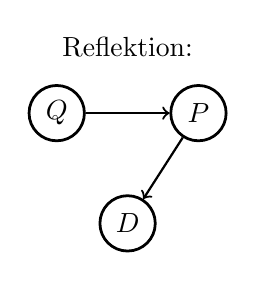
\begin{tikzpicture}
		\node[circle,draw=black,line width=1pt,inner sep=2pt,minimum size=20pt] (q) at (-.9,1.4) {$ Q $};
		\node[circle,draw=black,line width=1pt,inner sep=2pt,minimum size=20pt] (p) at (.9,1.4) {$ P $};
		\node[circle,draw=black,line width=1pt,inner sep=2pt,minimum size=20pt] (d) at (0,0) {$ D $};
		\draw[thick,->] (q) -- (p);
		\draw[thick,->] (p) -- (d);
		\node[above] at (0,2) {Reflektion:};
	\end{tikzpicture}
	\hspace{2cm}
	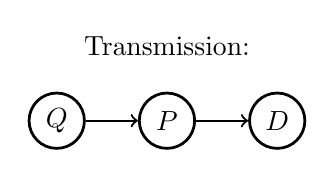
\begin{tikzpicture}
		\node[circle,draw=black,line width=1pt,inner sep=2pt,minimum size=20pt] (q) at (-1.4,0) {$ Q $};
		\node[circle,draw=black,line width=1pt,inner sep=2pt,minimum size=20pt] (p) at (0,0) {$ P $};
		\node[circle,draw=black,line width=1pt,inner sep=2pt,minimum size=20pt] (d) at (1.4,0) {$ D $};
		\draw[thick,->] (q) -- (p);
		\draw[thick,->] (p) -- (d);
		\node[above] at (0,.7) {Transmission:};
	\end{tikzpicture}
	\hspace{2cm}
	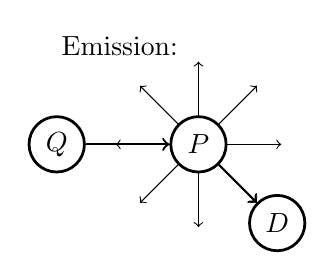
\begin{tikzpicture}
		\node[circle,draw=black,line width=1pt,inner sep=2pt,minimum size=20pt] (q) at (-1.8,0) {$ Q $};
		\node[circle,draw=black,line width=1pt,inner sep=2pt,minimum size=20pt] (p) at (0,0) {$ P $};
		\node[circle,draw=black,line width=1pt,inner sep=2pt,minimum size=20pt] (d) at (1,-1) {$ D $};
		\draw[thick,->] (q) -- (p);
		\draw[thick,->] (p) -- (d);
		\node[above] at (-1,1) {Emission:};
		\foreach \a in {0,45,90,135,180,225,270,315}
		\draw[->] (\a:10pt) -- ++(\a:.7cm);
	\end{tikzpicture}
\end{center}
\folie{Schematisch: Spektrometer}\\[5pt]
\versuch{Natrium-Dampf-Lampe}
Das Licht aus der Natrium-Dampf-Lampe geht durch eine Glasröhre mit aufgedampftem Natrium. Diese Röhre wird nun erhitzt, sodass das Natrium verdampft.
Aufgrund der Erhitzung wird das nun Gasförmige Natrium von der Lampe angeregt und Emittiert selbst auch Licht derselben Farbe. Da dieses Licht nicht mehr gerichtet ist sondern in alle Richtungen strahlt wird die Intensität des transmittierten Lichts geringer.\\
Bei sehr hoher Temperatur ist die Absorption so stark, dass nach dem Anfangsbereich der Röhre schon das ganze Licht Absorbiert und ausgestrahlt wird.\\[5pt]
\versuch{Weißes Licht auf Salz (Natriumchlorid)}
Sichtbares Spektrum: Rot$ | $Grün.\\
Emissionsspektrum über Erhitzung ohne Weißlicht-Beleuchtung mit Gasbrenner (farbige Flamme)\\
Bei Erhitzung und Beleuchtung: Absorptionsspektrum: Rot - Gelb - Grün.\\[5pt]
\versuch{Rayleigh Strahlung}
Eine Lampe strahlt unpolarisiertes Weißes Licht aus.\\
Das an den Wassermolekülen (und Dreckrückständen im Wasser) gestreute Licht hat eine lineare Polarisation. Von den Molekülen geht eine Herz'sche Dipolstrahlung aus (Polarisation in Richtung der Antenne, Ausbreitung der Welle in der Ebene orthogonal dazu). Dies kommt daher, dass das Weiße licht nur transversal polarisierte Anteile hat keine longitudinalen. Daraus ergibt sich, welche Dipole angeregt werden, und das die Polarisation nur orthogonal zur Ausbreitung des Lichts stattfindet.\\
Die Rayleigh-Streuung ist mit $ \omega^4 $ Frequenzabhängig, es wird also blau wesentlich stärker Reflektiert als rotes Licht.es Licht. Dies erklärt den Blauen Schimmer um die Weiße Kreisscheibe auf dem Schirm.\\
Beim hinzugeben von winzigen Kügelchen, die im Wasser schwimmen, wird mehr Licht gestreut. Die Kreisscheibe wird immer röter und röter zunächst gelb dann dunkel orange wie die Abendsonne. Die blauen Frequenzen sind eher am Rand zu sehen und konzentrierter als zuvor. (Beim blauen Himmel sehen wir den Emissionsanteil hier den Transmissionsanteil).\\[5pt]

\subsubsection{Typen von Spektren}

Linienspektrum \& kontinuierliches Spektrum\\
\folie{verschiedene Spektren}\\
\textbf{Zugängliche Infos im Linienspektrum (Prüfungsrelevant!)}
\begin{enumerate}[1)]
	\item Die Lage des Peaks oder die Frequenz des Peaks gibt die \textbf{Übergangsenergie} an die nur eine Energiedifferenz angibt.\\
	\begin{minipage}{.8\linewidth}
		\begin{equation*}
		E_2 - E_1 = kv
		\end{equation*}
	\end{minipage}%
	\begin{minipage}{.2\linewidth}
		%t3:
		\centering
		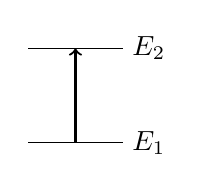
\begin{tikzpicture}[scale=.6]
			\draw (-1,1) -- (1,1) node[right] {$ E_2 $};
			\draw (-1,-1) -- (1,-1) node[right] {$ E_1 $};
			\draw[thick,->] (0,-1) -- (0,1);
		\end{tikzpicture}
	\end{minipage}%
	\item \textbf{Intensität}: Diese hängt von der Übergangswahrscheinlichkeit und damit auch der Teilchendichte zusammen.\\
	Die Intensität hat auch mit der \textbf{stärke der Wechselwirkung} von dem Eingestrahlten (\textbf{Sonde}) mit dem Bestrahlten (\textbf{Probe}) zu tun.
	\item \textbf{Linienbreite/Linienform:}	Bei der Lorenzverteilung ist die Breite der Verteilung verknüpft mit der Lebensdauer der Teilchen.
	\begin{equation*}
	e^{-\frac{t}{\tau}} \quad \Rightarrow \quad \tx{Lorenzlinie} \quad \Rightarrow \quad \tx{Lebensdauer}
	\end{equation*}
	\folie{Gaußverteilung als Summe der Wahrscheinlichkeitsverteilungen einzelner Moleküle}
	\begin{equation*}
	\tx{statistische Verteilung } \quad \Rightarrow \quad \tx{Gaußverteilung}
	\end{equation*}
\end{enumerate}

\section*{Fragerunde}
\addcontentsline{toc}{section}{IV. \texorpdfstring{\ \: }{space}  Fragerunde}

\textbf{Dispersionsrelation bei getriebener Schwingung:}\\
(harmonischer Oszillator oder Dispersion bei Schwingungen)\\
Gleichschwingung bei geringer Antriebsfrequenz.\\
Phasenverschiebung bei zu schnellem Antrieb und geringe Amplitude des Schwingers\\
quasi ein Tiefpass.\\
Dieses Problem ist mit komplexen Größen Lösbar. Zur Physikalischen Betrachtung der Lösung: Leistungsaufnahme des Schwingenden Systems. Diese Leistung ist mit dem Imaginärteil verknüpft.\\
Bei unserem Beispiel eines dielektrischen Materials geht es um Absorption. Diese stammt aus dem Leistungsverlust aus dem Imaginärteil der Dielektrizitätskonstante. Der Realteil ist hier mit dem Brechungsindex verknüpft.\\[5pt]
\textbf{Angeregte Emissionen:}\\
Das anregende und das angeregte Photon können aber müssen nicht in Phase sein. Allgemein ist dies nicht so.\\
Das angeregte Atom bleibt mit einer gewissen, statistisch verteilten Lebensdauer in dem Zustand. Wie die Anregung erfolgt ist (Stöße oder Absorption von Strahlung) ist egal. Daraus resultiert spontane Emission.\\
Die \textbf{stimulierte oder induzierte Emission} (erzeugt durch ein Strahlungsfeld) erzeugt die Abstrahlung von Photonen in Phase mit den eingestrahlten Photonen. Die Begründung ist recht kompliziert und kann nur über Quantenmechanik erfolgen.\\[5pt]
\textbf{Evaneszente Welle:}\\
Undurchdringbarkeit ist nur eine Näherung. Kein Wechsel des Mediums ist eine echte Stufenfunktion (im mikroskopischen Bereich).

% Vorlesung 5.12.18 (19 days untis christmas)

\section{Ratengleichungen}

\subsection{Exponentieller Zerfall}

\begin{equation*}
\prd{}{t} n(t) = - \frac{1}{\tau} [n(t) - n_{eq} ]
\end{equation*}
\lcom{Statistisch unabhängige Prozesse. Egal wie viele Objekte es gibt nach der Halbwertszeit ist nur noch die Hälfte da. Die einzelnen Objekte verhalten sich also unabhängig voneinander so.}\\
$ \tau : $ Radiationszeit, Zerfallszeit, Lebensdauer, Halbwertszeit, \dots\\
\textbf{Lösung:}
\begin{equation*}
n(t) = [n(o) - n_{eq}] e^{-\frac{t - t_0}{\tau}} + n_{eq}
\end{equation*}

\subsection{Zwei-Niveausystem}

\begin{center}
	%t1:
	\begin{tikzpicture}
		\coordinate (u) at ($ (0,0) + (0,1) $);
		\coordinate (d) at ($ (0,0) + (0,-1) $);
		\draw ($ (u) + (-1.5,0) $) node[left] {1} -- ++(3,0) node[right] {$ E_1 $};
		\draw ($ (d) + (-1.5,0) $) node[left] {0} -- ++(3,0) node[right] {$ E_0 $};
		\draw[red,thick,->] ($ (d) - (.5,0) $) to[out=110,in=-110] node[left] {$ \Gamma_{0\to1} $} ($ (u) - (.5,0) $);
		\draw[red,thick,->] ($ (u) + (.5,0) $) to[out=-70,in=70] node[right] {$ \Gamma_{1\to0} $} ($ (d) + (.5,0) $);
		\node[black!40!green] at ($ (u) + (2.5,0) $) {$ n_1 $};
		\node[black!40!green] at ($ (d) + (2.5,0) $) {$ n_0 $};
		\node[right,black!40!green] at (2.2,0) {Besetzungszahlen};
	\end{tikzpicture}
\end{center}
\emph{Bemerkung:}
\begin{itemize}
	\item oft gibt es eine \textbf{Zwangsbedingung} $ \sum_k n_k = N \quad N : $ Gesamtzahl der Zustände
	\item Prinzip des detaillierten Gleichgewichts
	\begin{equation*}
	\Gamma_{k \to l} = \Gamma_{l \to k}
	\end{equation*}
\end{itemize}
Ratengleichung:
\begin{equation*}
\dot{n}_0 = - \Gamma_{0 \to 1} n_0 + \Gamma_{1 \to 0} n_1
\end{equation*}
\begin{equation*}
\dot{n}_1 = - \Gamma_{1 \to 0} n_1 + \Gamma_{0 \to 1} n_0
\end{equation*}
Definition Gleichgewicht
\begin{align*}
\Rightarrow \quad \dot{n}_0 &= - \Gamma(n_0 - n_1) \\
\dot{n}_1 &= - \Gamma (n_1 - n_0)
\end{align*}
konstante Gesamtbesetzung
\begin{equation*}
n_0 + n_1 = N
\end{equation*}
\textbf{Lösung:}
\begin{align*}
\delta N \equiv n_1 - n_0 \qquad \rightarrow \quad n_0 &= \frac{1}{2} (N - \delta N) \\
n_1 &= \frac{1}{2} (N + \delta N)
\end{align*}
\begin{equation*}
\Rightarrow \quad - \frac{1}{2} \delta \dot{N} = \Gamma \delta N
\end{equation*}
\begin{equation*}
\delta N(t) = \delta N(0) e^{-\frac{t}{\tau}}
\end{equation*}

\subsubsection{Rantengleichung mit externen Stimuli}

\begin{minipage}{.5\linewidth}
	\begin{align*}
	\Rightarrow \quad \dot{n}_0 &= - \Gamma_{n_0} + \Gamma_{n_1} + \Gamma_{0 \tx{ext}}\\
	\dot{n}_1 &= - \Gamma_{n_1} + \Gamma_{n_0} + \Gamma_{1 \tx{ext}}
	\end{align*}
\end{minipage}%
\begin{minipage}{.5\linewidth}
	%t2:
	\centering
	\begin{tikzpicture}
		\coordinate (u) at ($ (0,0) + (0,1) $);
		\coordinate (d) at ($ (0,0) + (0,-1) $);
		\draw ($ (u) + (-1.5,0) $) node[left] {1} -- ++(3,0) node[right] {$ n_1 $};
		\draw ($ (d) + (-1.5,0) $) node[left] {0} -- ++(3,0) node[right] {$ n_0 $};
		\draw[red,thick,->] ($ (d) - (.5,0) $) to[out=110,in=-110] node[left] {$ \Gamma_{0\to1} $} ($ (u) - (.5,0) $);
		\draw[red,thick,->] ($ (u) + (.5,0) $) to[out=-70,in=70] node[right] {$ \Gamma_{1\to0} $} ($ (d) + (.5,0) $);
		\draw[<-] ($ (u) + (1.25,0) $) to[out=60,in=180] (2.5,2) node[right] {$ \Gamma_{1\tx{ ext}} $};
		\draw[<-] ($ (d) + (1.25,0) $) to[out=-60,in=180] (2.5,-2) node[right] {$ \Gamma_{0\tx{ ext}} $};
	\end{tikzpicture}
\end{minipage}%

\subsection{Zwei-Niveau System im Strahlungsfeld, Einstein Parameter}

\begin{minipage}{.5\linewidth}
	Im Folgenden Betrachten wir stets ein Zwei-Niveau-System wie hier in der Abbildung zu sehen ist:
\end{minipage}%
\begin{minipage}{.5\linewidth}
	%t3:
	\centering
	\begin{tikzpicture}
		\coordinate (u) at ($ (0,0) + (0,.8) $);
		\coordinate (d) at ($ (0,0) + (0,-.8) $);
		\draw ($ (u) + (-1.5,0) $) node[left] {1} -- ++(3,0) node[right] {$ E_1 , n_1 $};
		\draw ($ (d) + (-1.5,0) $) node[left] {0} -- ++(3,0) node[right] {$ E_0 , n_0 $};
	\end{tikzpicture}
\end{minipage}%
\\[15pt]
\textbf{spontane Emission:}\\
\begin{minipage}{.5\linewidth}
	\begin{align*}
	\Rightarrow \quad \dot{n}_1 &= - A_{1 \to 0} n_1 \\
	\dot{n}_0 &= + A_{1 \to 0} n_1
	\end{align*}
\end{minipage}%
\begin{minipage}{.5\linewidth}
	%t4:
	\centering
	\begin{tikzpicture}
		\coordinate (u) at ($ (0,0) + (0,.8) $);
		\coordinate (d) at ($ (0,0) + (0,-.8) $);
		\draw ($ (u) + (-1.5,0) $) -- ++(3,0);
		\draw ($ (d) + (-1.5,0) $) -- ++(3,0);
		\draw[red,thick,->] (u) -- (d);
		\draw[red,thick,->,decorate,decoration=snake] (0.5,0) -- (2.2,0) node[right] {$ h \nu $};
	\end{tikzpicture}
\end{minipage}%
\\[15pt]
\textbf{Photon Absorption:}\\
\begin{minipage}{.5\linewidth}
	\begin{align*}
	\Rightarrow \quad \dot{n}_0 &= - B_{0 \to 1} \rho(\nu) n_0 \\
	\dot{n}_1 &= + B_{0 \to 1} \rho(\nu) n_0
	\end{align*}
\end{minipage}%
\begin{minipage}{.5\linewidth}
	%t5:
	\centering
	\begin{tikzpicture}
		% ugly invisibe alignment line
		\draw[white] (0,0) -- (4.1,0);
		\coordinate (u) at ($ (0,0) + (0,.8) $);
		\coordinate (d) at ($ (0,0) + (0,-.8) $);
		\draw ($ (u) + (-1.5,0) $) -- ++(3,0);
		\draw ($ (d) + (-1.5,0) $) -- ++(3,0);
		\draw[red,thick,->] (d) -- (u);
		\draw[red,thick,->,decorate,decoration=snake] (-2.7,0) -- (-1,0) node[right] {$ h \nu $};
	\end{tikzpicture}
\end{minipage}%
\\[15pt]
$ \rho(\nu) : $ Dichte des Strahlungsfeldes\\
$ \nu : $ Frequenz\\[5pt]
\textbf{stimulierte Emission:}\\
\begin{minipage}{.5\linewidth}
	\begin{align*}
	\Rightarrow \quad \dot{n}_0 &= + B_{1 \to 0} \rho(\nu) n_1 \\
	\dot{n}_1 &= - B_{1 \to 0} \rho(\nu) n_1
	\end{align*}
\end{minipage}%
\begin{minipage}{.5\linewidth}
	%t6:
	\centering
	\begin{tikzpicture}
		% ugly invisibe alignment line
		\draw[white] (0,0) -- (3.2,0);
		\coordinate (u) at ($ (0,0) + (0,1) $);
		\coordinate (d) at ($ (0,0) + (0,-1) $);
		\draw ($ (u) + (-1.5,0) $) -- ++(3,0);
		\draw ($ (d) + (-1.5,0) $) -- ++(3,0);
		\draw[red,thick,->] (u) -- (d);
		\draw[red,thick,->,decorate,decoration=snake] (-1.8,0) -- node[above] {$ h \nu $} (-.1,0);
		\draw[red,thick,->,decorate,decoration=snake] (0.1,.4) -- (1.8,.4);
		\draw[red,thick,->,decorate,decoration=snake] (0.1,-.4) -- (1.8,-.4) node[right,yshift=12pt] {$ h \nu $};
	\end{tikzpicture}
\end{minipage}%
\\[15pt]
\textbf{Definition Gleichgewicht}
$ n_0 : $
\begin{equation*}
A_{1 \to 0} n_1 - B_{0 \to 1} \rho(\nu) n_0 + B_{1 \to 0} \rho(\nu) n_1 = 0
\end{equation*}
Thermodynamik, Quantenstatistik:
\begin{equation*}
\frac{n_k}{N} = \frac{1}{Z} e^{-\frac{E_k}{k_B T}}
\end{equation*}
\begin{equation*}
\rho(\nu) = \frac{8 \pi h \nu^3}{c^3} \frac{1}{e^{\frac{h \nu}{k_B T}} - 1}
\end{equation*}
$ Z : = \sum_k e^{-\frac{E_k}{k_B T}} $ die Zustandssumme\\
$ k_B : $ Boltzmann-Konstante\\[5pt]
$ \Rightarrow $ Planck'sches Strahlungsgesetz